% THIS DOCUMENT IS FOLLOWS THE VOLERE TEMPLATE BY Suzanne Robertson and James Robertson
% ONLY THE SECTION HEADINGS ARE PROVIDED
%
% Initial draft from https://github.com/Dieblich/volere
%
% Risks are removed because they are covered by the Hazard Analysis
\documentclass[12pt]{article}

\usepackage{booktabs}
\usepackage{tabularx}
\usepackage{hyperref}
\usepackage{graphicx}
\usepackage{caption}
\usepackage{enumitem}
\usepackage{float}
\usepackage{longtable}
\usepackage[english]{babel}
\usepackage[acronym,nonumberlist]{glossaries}

\hypersetup{
    bookmarks=true,         % show bookmarks bar?
      colorlinks=true,      % false: boxed links; true: colored links
    linkcolor=red,          % color of internal links (change box color with linkbordercolor)
    citecolor=green,        % color of links to bibliography
    filecolor=magenta,      % color of file links
    urlcolor=cyan           % color of external links
}

\makenoidxglossaries
\newacronym{mes}{MES}{McMaster Engineering Society}
\newacronym{cfes}{CFES}{Canadian Federation of Engineering Students}
\newglossaryentry{adm}{
  name=admin,
  description={A privileged system user affiliated with \gls{mes} who can access survey, event, and attendee records;
  track finances; and update event statuses.}
  plural=admins,
}
\newglossaryentry{atd}{
  name=attendee,
  description={An individual who attends an \gls{mes} event, and uses the system to register, receive event updates,
  provide feedback, or fill out survey responses.}
  plural=attendees,
}

\newcommand{\lips}{\textit{Insert your content here.}}
\newcolumntype{Y}{>{\raggedright\arraybackslash}X}
\newcolumntype{P}[1]{>{\centering\arraybackslash}p{#1}}
\renewcommand{\glossarysection}[2][]{}

%% Comments

\usepackage{color}

\newif\ifcomments\commentstrue %displays comments
%\newif\ifcomments\commentsfalse %so that comments do not display

\ifcomments
\newcommand{\authornote}[3]{\textcolor{#1}{[#3 ---#2]}}
\newcommand{\todo}[1]{\textcolor{red}{[TODO: #1]}}
\else
\newcommand{\authornote}[3]{}
\newcommand{\todo}[1]{}
\fi

\newcommand{\wss}[1]{\authornote{magenta}{SS}{#1}} 
\newcommand{\plt}[1]{\authornote{cyan}{TPLT}{#1}} %For explanation of the template
\newcommand{\an}[1]{\authornote{cyan}{Author}{#1}}

%% Common Parts

\newcommand{\progname}{Software Engineering} % PUT YOUR PROGRAM NAME HERE
\newcommand{\teamname}{EvENGage}
\newcommand{\authname}{Team 4, \teamname
\\ Virochaan Ravichandran Gowri
\\ Omar Al-Asfar
\\ Rayyan Suhail
\\ Ibrahim Quraishi
\\ Mohammad Mahdi Mahboob} % AUTHOR NAMES

\newcommand{\prjdesc}{MES Event Management Registration, Administration, and Survey Analytics}

\usepackage{hyperref}
    \hypersetup{colorlinks=true, linkcolor=blue, citecolor=blue, filecolor=blue,
                urlcolor=blue, unicode=false}
    \urlstyle{same}



\begin{document}

\title{Software Requirements Specification for \progname: A Platform for Event Management }
\author{\authname}
\date{\today}

\maketitle
~\newpage

\tableofcontents

~\newpage

\section*{Revision History}

\begin{tabularx}{\textwidth}{p{3cm}p{2cm}X}
\toprule {\textbf{Date}} & {\textbf{Version}} & {\textbf{Notes}}\\
\midrule
Date 1 & 1.0 & Notes\\
Date 2 & 1.1 & Notes\\
\bottomrule
\end{tabularx}

~\\

~\newpage
\section{Purpose of the Project}

The purpose of this project is to create a centralized platform for the \gls{mes} that simplifies how large-scale events
are managed. By consolidating event registration, form creation, attendee tracking, and data analytics into a single
system, the platform aims to reduce administrative workload, eliminate fragmented workflows, and enhance the overall
experience for both event organizers and attendees.

\subsection{User Business}

The primary users of this system are members of the McMaster Engineering Society, including executives and event
organizers, as well as McMaster engineering students who attend \gls{mes} events.

\begin{itemize}
    \item \textbf{Administrators (\gls{mes} Executives and Organizers):} Responsible for creating events, designing
      registration and feedback forms, managing attendee information, and analyzing data through the dashboard. They
      will use the platform to reduce manual work and improve event coordination.
    \item \textbf{End Users (Students and Attendees):} Students will use the platform to register for events, complete
      waivers or feedback forms, and receive event confirmations and updates. The goal is to create a seamless and
      engaging experience that encourages participation.
\end{itemize}

By serving both groups through a single platform, the system eliminates redundant workflows and ensures continuity of
data across multiple events.

\subsection{Goals of the Project}

The primary goals of this project are as follows:

\begin{enumerate}
    \item \textbf{Develop a Custom Form Builder:} Build an intuitive tool that lets administrators design and manage
      event or feedback forms with different question types and conditional logic, without needing third-party software.
    \item \textbf{Implement a Unified Registration and Feedback System:} Create a simple, centralized process for
      students to register for events, complete waivers, and share feedback—all in one place.
    \item \textbf{Create an Attendee Overview Dashboard:} Give administrators a clear view of event participation by
      displaying key details such as registration status, payments, and waiver completion in real time.
    \item \textbf{Integrate Backend Analytics:} Include tools that help \gls{mes} organizers analyze event data, track
      trends, and use insights to plan and improve future events more effectively.
\end{enumerate}



\section{Stakeholders}
\subsection{Client}
The client for this project is the supervisor, Luke Schuurman. He is a member of the \gls{mes} and has first-hand
experience planning and hosting events with the \gls{mes}. As the supervisor he will play a crucial role by ensuring the
project aligns with objective of the \gls{mes} and integrate the platform seamlessly with existing systems. He will also
provide us with feedback and guidance throughout the project and will help define the project requirements in this
document.
% \subsection{Customer}
% \lips
% \subsection{Other Stakeholders}
% \lips
\subsection{Hands-On Users of the Project}
\textbf{\gls{mes} Executives and Council Members}: They will be utilizing this system to create and manage events,
configure forms and surveys, monitor event data and generate data analytics reports. They can be characterized as
primarily undergraduate students who value their time greatly. They aim to reduce the time taken to do administrative
tasks as well as provide a better experience during \gls{mes} events. Their experience with systems like this can range
from Journeyman - Master as they can be experienced in event planning and student engagement. There may be a slight
learning curve to utilizing the new technology, but these users have experience performing these functions.\\
\newline
\textbf{McMaster Engineering Students}: They will be utilizing this app to register for events, purchase tickets, sign
waivers, check in at venues, and complete feedback surveys. They want to enjoy their university experience and connect
with other students, They are also very busy and value their time greatly so are looking for an intuitive and
straightforward user experience. Their general experience with systems like this is Journeyman as they may have used
similar systems for other use cases. \\
\newline
\textbf{Other Students and Guest Event Attendees}: This group includes non-engineering students, alumni, and invited
guests who participate in large-scale \gls{mes} events such as the Fireball Formal and Graduation Formal, which extend
beyond the core engineering community. It could also include students and guests from other universities as well as
industry which attend the engineering conferences that the \gls{mes} helps host. They are generally looking for an easy
and seamless experience registering and attending these events. Their general experience with systems like this is
Journeyman as they may have used similar systems for other use cases.
\subsection{Personas}
\begin{enumerate}
  \item \textbf{Matthew Cruise (Engineering Student)}: Matthew is a 20-year-old second-year Mechanical Engineering
    student at McMaster University. He lives in a shared house near campus with two close friends. He enjoys attending
    \gls{mes} events like pub nights and the Fireball Formal as a way to balance his heavy academic workload with some
    enjoyment and entertainment. He usually hears about events through word-of-mouth or social media and would prefer an
    easy and effortless way to find and register for events. Matthew is generally tech-savvy and is comfortable using
    online platforms but doesn't want to be bothered by too many notifications and forms. He has many ideas on how he
    can generally improve his university experience but doesn't believe he has an outlet to convey them. For Matthew his
    priority is convenience as he wants to enjoy himself but doesn't want to spend too much time or effort doing so.
  \item \textbf{Adam Clooney (\gls{mes} Executive)}: Adam Clooney is a 22-year-old final-year Civil Engineering student
    who currently serves as VP Social on the \gls{mes}. He is responsible for coordinating large-scale events like
    Fireball Formal, working closely with other council members to handle logistics, advertising, and student
    engagement. Adam is outgoing and enjoys bringing people together, but often feels the strain of balancing his role
    with academic responsibilities. He is proficient with common digital tools such as Google Drive, spreadsheets, and
    design platforms for promotions, but he’s not highly technical. Adam appreciates structure and tools that keep
    things organized because he dislikes wasting time fixing errors or repeating work. He is motivated by the sense of
    accomplishment that comes from hosting a successful event and wants tools that help him stay on top of details.
  \item \textbf{Margot Watson (McMaster Student)}: Margot Watson is a 21-year-old undergraduate student in Political
    Science at McMaster University. Although she is not part of the engineering faculty, she often attends large
    \gls{mes}-hosted events such as the Fireball Formal and other socials because many of her friends are in
    engineering. Margot lives in an off-campus apartment with two roommates and enjoys being involved in student life
    across faculties. She has a relaxed attitude toward technology since she uses her phone daily for social media and
    messaging, but she prefers things to be straightforward and intuitive. She is cautious with her money, balancing
    tuition and living expenses, but she’s willing to spend on experiences with friends. She is motivated by spending
    time with her friends and having good experiences to have a fulfilling student life.
\end{enumerate}
\subsection{Priorities Assigned to Users}
\textbf{Key Users:} Luke Schuurman, \gls{mes} Council Members and Executives, McMaster Engineering Students. \\
\textbf{Secondary Users:} Other Students and Guest Event Attendees.
\subsection{User Participation}
Our requirements will primarily be derived through meetings with our supervisor Luke Schuurman. If we have the need to
clarify or elicit more requirements we will look to engage other \gls{mes} members either through our supervisor or
directly.

% \subsection{Maintenance Users and Service Technicians}
% \lips

\section{Mandated Constraints}
\subsection{Solution Constraints}
\lips
\subsection{Implementation Environment of the Current System}
\lips
\subsection{Partner or Collaborative Applications}
\lips
\subsection{Off-the-Shelf Software}
\lips
\subsection{Anticipated Workplace Environment}
\lips
\subsection{Schedule Constraints}
\lips
\subsection{Budget Constraints}
\lips
\subsection{Enterprise Constraints}
\lips

\section{Naming Conventions and Terminology}
\subsection{Glossary of All Terms, Including Acronyms, Used by Stakeholders
involved in the Project}
\glsaddall
\printnoidxglossaries

\section{Relevant Facts And Assumptions}

\subsection{Relevant Facts}

\begin{itemize}
    \item The McMaster Engineering Society currently manages events such as Fireball Formal and the CALE Conference
      using several disconnected tools like Google Forms and Google Sheets, which creates inefficiencies and limits data
      analysis.
    \item Each \gls{mes} event involves registration, waiver collection, and feedback surveys that must comply with
      university data privacy and accessibility standards.
    \item The system will be used by both administrators and students on a wide range of devices and browsers, so
      responsive and cross-platform design is required.
    \item The overall Event Management System is being co-developed by three Capstone teams. Project A must maintain
      compatibility and shared data models with the other two teams’ components.
    \item The project’s frontend stack was recently updated from \textbf{Next.js} to \textbf{Vite + TanStack Router +
      TanStack Create} to improve development speed, hot reloading performance, and flexibility for building a Single
      Page Application (SPA) with integrated admin dashboards and authentication.
    \item PostgreSQL remains the chosen database technology for data storage and analytics.
\end{itemize}

\subsection{Business Rules}

\begin{itemize}
    \item Only verified \gls{mes} administrators can create, edit, or delete forms and view backend analytics.
    \item Event data, form responses, and attendee details must be securely stored and retrievable for future event
      reviews.
    \item All user input will be validated to prevent incomplete or invalid submissions before being stored in the
      database.
    \item A consistent data format must be maintained across all events to support accurate analytics and report
      generation.
    \item Administrators can export data such as attendee lists or analytics summaries in standard formats (e.g., CSV,
      PDF).
\end{itemize}

\subsection{Assumptions}

\begin{itemize}
    \item The \gls{mes} will provide sample event and registration data to support development and testing.
    \item Users will have stable internet access when using the platform, as it relies on real-time connectivity.
    \item Collaborating teams (Projects B and C) will follow the agreed API and database specifications to ensure system
      integration works smoothly.
    \item Authentication and authorization will be handled securely within the shared platform using standardized
      methods.
    \item Future \gls{mes} administrators and developers will continue maintaining the project using the provided GitHub
      repository, documentation, and CI/CD workflows.
\end{itemize}

\section{The Scope of the Work}

The purpose of the section is to define the expected scope of the project, including specifications on how the system is
partitioned, business data models, and business use cases.

\subsection{The Current Situation}

Currently, the \gls{mes} uses plethora of different platforms to host events and conduct surveys such as tools for
registration, signing of waivers, and checking in \glspl{atd}. The main platforms used are a combination of Google Forms
and Google Sheets. There are several pain points to address with the current system.

\begin{itemize}
  \item \textbf{Decentralized System Components} Registration and surveying is split across a plethora of tools and
    software which may not be compatible with each other. For example, Google Forms is used for registration forms and
    surveys, Google Sheets stores form data and LinkTree holds links to all the registration forms, and event updates is
    done by email or social media.
  \item \textbf{Overly Complex Form Logic} The current \gls{cfes} survey consists of 70 pages of questions linked
    together through complex branching logic. The Google Forms form building UI makes this very complicated as all form
    elements are displayed as a linear list of sections making it very hard to track paths through the form.
  \item \textbf{Disorganized Data Visualization} Form response data is currently stored using Google Sheets. While
    Google Form data is easily imported into Google Sheets, any analytics on the data must be done manually through
    equations and macros.
  \item \textbf{Lack of Reusability} Google Forms comes with a few templates that provide an initial starting point for
    many types of forms such as registrant information. However, after the first section of the form, each subsequent
    section must be made manually. Sections may be imported from other forms, but this requires the user to have access
    to a form with the wanted section and to scour through an unorganized list of forms and sections.
  \item \textbf{Low Response Rates on Surveys} The response rates on the annual \gls{cfes} survey of undergraduate engineering
    students have been decreasing due to the long length of the Google Form and the lack of ability to submit a
    partially completed form.
  \item \textbf{Manual Registration Scheduling} Event registration is managed through a combination of Instagram, Google
    Forms, and LinkTree. Events are advertised on Instagram, and a link to the signup Google Form is posted on the
    \gls{mes} LinkTree. This solution lacks automation since a new Google Form must be made for every event and links
    have to be manually added and removed for each form when registration is opened or closed.
\end{itemize}

% \gls{mes} hosts lots of events per year
% Their event management system is unorganized
% Consists of google forms, google sheets
% No template form to work with redundant info between forms like name, number email, etc
% Lots of steps to registration and split across too many platforms
% The same thing is done for the annual \gls{cfes} survey of undergrad eng students
% long 70 page form of complex branching logic, low response rate
%


\subsection{The Context of the Work}

This section provides an overview of the high-level inputs and outputs between the system and external systems or
actors.
The system is split into two perspectives, the \gls{atd} perspective shown in \hyperref[fig:workcontextuser]{Figure
\ref{fig:workcontextuser}}, and the \gls{adm} perspective shown in \hyperref[fig:workcontextadmin]{Figure
\ref{fig:workcontextadmin}}.

\begin{center}
\begin{figure}[H]
    \centering
    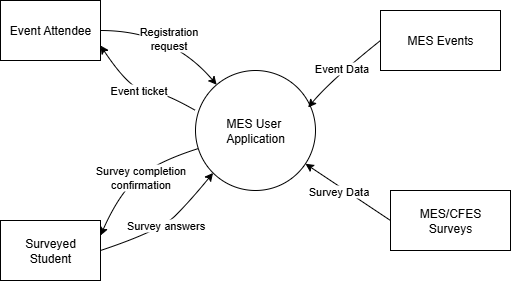
\includegraphics[width=1\linewidth]{images/work_context_user.png}
    \caption{Work context diagram of the \gls{atd} side application}\label{fig:workcontextuser}
\end{figure}
\end{center}

\begin{center}
\begin{figure}[H]
    \centering
    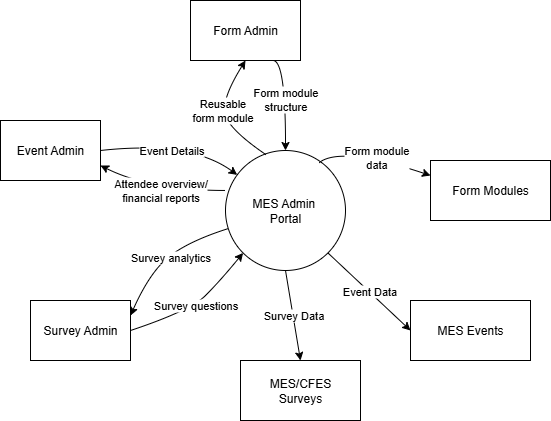
\includegraphics[width=1\linewidth]{images/work_context_admin.png}
    \caption{Work context diagram of the \gls{adm} side application}\label{fig:workcontextadmin}
\end{figure}
\end{center}

\subsection{Work Partitioning}

This section describes how the work done by the system can be partitioned into smaller and more manageable workflows.
Below is a table describing each of the sub-workflows of the proposed systems. Note that event creation and survey
creation have been grouped as a single workflow since they are nearly identical.

{
  \setlength{\tabcolsep}{0.125em}
  \renewcommand{\arraystretch}{1.2}
  \begin{table}[H]
    \centering
    \begin{tabularx}{\textwidth}{|P{2.5em}|Y|Y|Y|Y|}
      \hline
      \textbf{No.} & \textbf{Event} & \textbf{Input} & \textbf{Output} & \textbf{Requirements} \\ \hline
      1 & \Gls{atd} registers for event & Registration data & Event ticket & \\ \hline
      2 & \Gls{atd} fills out a survey & Survey responses & Survey completion confirmation & \\ \hline
      3 & \Gls{adm} creates a form module & Module question data & Reusable form module & \\ \hline
      4 & \Gls{adm} creates an event/survey & Event/survey data & Event/survey creation confirmation & \\ \hline
      5 & \Gls{adm} views survey/event statistics & Event/survey to view & Event/survey registration/response reports &
      \\ \hline
    \end{tabularx}
    \captionof{table}{Partitioning of system workflows}\label{wfpart}
  \end{table}
}

\subsection{Specifying a Business Use Case (BUC)}

\subsubsection*{BUC 1: User registers for an event}
\textbf{Input:} Registration data \\
\textbf{Output:} Event tickets \\
\textbf{Pre-condition:} User has downloaded the application and has created an account \\
\textbf{Scenario:}
\begin{enumerate}
  \item The user application receives the registration data
  \item The user application verifies the data is filled correctly
  \item The user application sends the registration data to the backend server
  \item The backend server verifies the event is not full, and the deadline has not passed
  \item The backend server adds the user to the list of \glspl{atd}
  \item The backend server generates an event ticket and sends it to the user application
  \item The user application confirms with the user that the registration was successful and presents the user with the
    ticket
\end{enumerate}
\textbf{Sub variations:}
\begin{itemize}
  \item [2a.] The submitted registration data has errors: the user application prompts the user to fix the errors and resubmit.
  \item [4a.] The event is full, or the deadline has passed: the backend sends an error code to the user application.
  \item [4b.] The user application alerts the user of the error.
\end{itemize}

\subsubsection*{BUC 2: User fills out a survey module}
\textbf{Input:} Survey responses \\
\textbf{Output:} Survey completion confirmation \\
\textbf{Pre-condition:} \Gls{atd} has downloaded the application and has created an account \\
\textbf{Scenario:}
\begin{enumerate}
  \item The user application receives the survey data
  \item The user application verifies the data is filled correctly
  \item The user application sends the survey data to the backend server
  \item The backend server updates the survey database with the \gls{atd}'s data
  \item The backend server sends a confirmation message to the user application
  \item The user application confirms with the \gls{atd} that the survey data has been submitted
\end{enumerate}
\textbf{Sub variations:}
\begin{itemize}
  \item [2a.] The submitted data has errors (i.e. mandatory fields not filled), the user application prompts the \gls{atd} to fix the errors and resubmit
\end{itemize}

\subsubsection*{BUC 3: \Gls{adm} creates a form module}
\textbf{Input:} Form fields \\
\textbf{Output:} Reusable form module \\
\textbf{Pre-condition:} \Gls{adm} has access to create custom form modules \\
\textbf{Scenario:}
\begin{enumerate}
  \item The \gls{adm} portal receives the list of form fields and questions from the \gls{adm} user for the custom module
  \item The \gls{adm} portal verifies the custom module has been created correctly
  \item The \gls{adm} portal sends the custom module data to the backend server
  \item The backend server authenticates the \gls{adm} user
  \item The backend server saves the custom module data to the template database
  \item The backend server sends a confirmation message to the \gls{adm} portal
  \item The \gls{adm} portal updates the list of custom modules with the completed module
  \item The \gls{adm} portal confirms with the \gls{adm} user that the custom module has been created
\end{enumerate}
\textbf{Sub variations:}
\begin{itemize}
  \item [2a.] The submitted form module has errors (i.e. unfinished fields), the \gls{adm} user is prompted to fix these errors before resubmitting
  \item [4a.] Authentication of the \gls{adm} fails, the \gls{adm} portal is notified of the request denial
\end{itemize}

\subsubsection*{BUC 4: \Gls{adm} creates an event/survey}
\textbf{Input:} Event details \\
\textbf{Output:} Event creation confirmation \\
\textbf{Pre-condition:} \Gls{adm} has access to create events \\
\textbf{Scenario:}
\begin{enumerate}
  \item The \gls{adm} portal receives the event/survey details
  \item The \gls{adm} portal verifies the event/survey details are correct
  \item The \gls{adm} portal sends the event/survey data to the backend server
  \item The backend server authenticates the \gls{adm} user
  \item The backend server saves the event/survey data to the database of events/surveys
  \item The backend server sends a message to the user application to notify users of the new event/survey
  \item The backend server sends a confirmation message to the \gls{adm} portal
  \item The \gls{adm} portal adds the created event/survey to the event/survey dashboard
  \item The \gls{adm} portal confirms with the \gls{adm} user that the event/survey has been created
\end{enumerate}
\textbf{Sub variations:}
\begin{itemize}
  \item [2a.] The submitted details have errors (i.e. event date has already passed), the \gls{adm} user is prompted to fix these errors before resubmitting
  \item [4a.] Authentication of the \gls{adm} fails, the \gls{adm} portal is notified of the request denial
\end{itemize}

\subsubsection*{BUC 5: \Gls{adm} views event/survey statistics}
\textbf{Input:} Event/survey to view \\
\textbf{Output:} Event registration/survey response report \\
\textbf{Pre-condition:} Event/survey has been created, and \glspl{atd} have registered/responded \\
\textbf{Scenario:} \\
\begin{enumerate}
  \item The admin portal receives the request to view event/survey statistics
  \item The admin portal sends a request to the backend server containing the identification for the event/survey to view
  \item The backend server receives the request and authenticates the \gls{adm}
  \item The backend server retrieves the registrant/response data for the requested event/survey from the database
  \item The backend server generates a statistical report of all the data
  \item The data is sent back to the admin portal
  \item The admin portal formats all the data into a readable format
  \item The \gls{adm} is presented with the event/survey statistics
\end{enumerate}
\textbf{Sub variations:}
\begin{itemize}
  \item [3a.] Authentication of the \gls{adm} fails, the admin portal is notified of the request denial
\end{itemize}

\section{Business Data Model and Data Dictionary}

The purpose of this section is to illustrate the flow of data throughout the system.

\subsection{Business Data Model}

\hyperref[fig:businessdata]{Figure \ref{fig:businessdata}} splits the system into into well defined subsystems and outlines the interactions between subsystems.

\begin{center}
\begin{figure}[H]
    \centering
    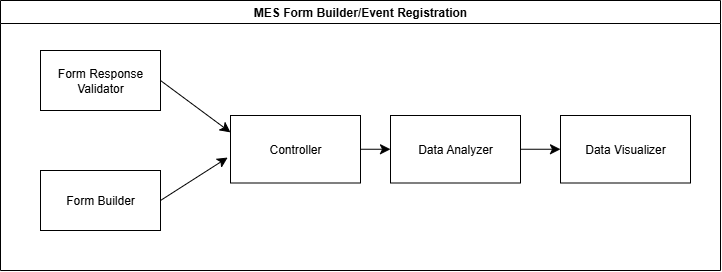
\includegraphics[width=1\linewidth]{images/business_data_model.png}
    \caption{Diagram of the interactions between main system components}\label{fig:businessdata}
\end{figure}
\end{center}
\subsection{Data Dictionary}

\hyperref[table:datadictionary]{Table \ref{table:datadictionary}} defines each of the system components shown in \hyperref[fig:businessdata]{Figure \ref{fig:businessdata}}.
{
\setlength{\tabcolsep}{0.3em}
\renewcommand{\arraystretch}{1.2}
\begin{table}[H]
    \begin{tabular}{p{0.25\linewidth}p{0.6\linewidth}p{0.2\linewidth}}
      \toprule
      \textbf{Component Name}              & \textbf{Description}                                                                                                                                       & \textbf{Type} \\ \midrule
        \gls{mes} Event/Survey Manager             & The application handling the \gls{adm} side of the system, including event/survey creation, and data analytics                                                 & Application   \\ \midrule
        Event Builder                        & Contains tools for creating, publishing, and managing events                                                                                               & Module        \\ \midrule
        Survey Builder                       & Contains tools for creating, publishing, and managing surveys                                                                                              & Module        \\ \midrule
        Admin Controller                     & Handles the flow of execution of \gls{mes} Event/Survey Manager modules and data flow between the event/survey builders, data analyzers, and the user controller & Module        \\ \midrule
        Financial Analyzer                   & Automates analysis and visualization of finances from event attendee data                                                                                  & Module        \\ \midrule
        Survey Analyzer                      & Automates analysis and visualization of survey response data                                                                                               & Module        \\ \midrule
        \gls{mes} Event Registration/Survey Filler & The application handling the \gls{atd} side of the system, including event registration and survey responses                                                    & Application   \\ \midrule
        Form Filler                          & Handles input and validation of form responses                                                                                                             & Module        \\ \midrule
        User Controller                      & Controls the flow of execution of the form filler and handles communication with the admin controller                                                      & Module        \\ \midrule
    \end{tabular}
    \captionof{table}{Data dictionary table}\label{table:datadictionary}
\end{table}
}

\section{The Scope of the Product}

The purpose of this section is to define the scope of the product by defining the boundaries of each major component of the system as well as their functionalities, interfaces for external actors, and interactions with each other.

\subsection{Product Boundary}

\hyperref[fig:productusecase]{Figure \ref{fig:productusecase}} outlines the main components of the system, how they interact with each other, and their related use cases.

\begin{center}
\begin{figure}[H]
    \centering
    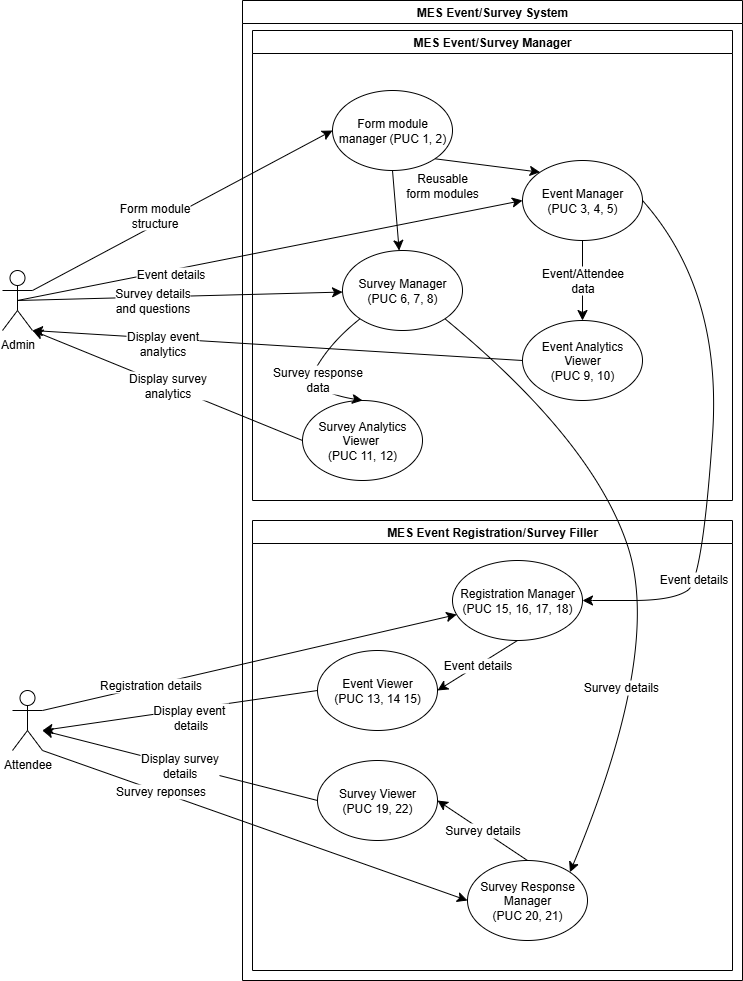
\includegraphics[width=0.89\linewidth]{images/product_use_case.png}
    \caption{Product use case diagram}\label{fig:productusecase}
\end{figure}
\end{center}
\subsection{Product Use Case Table}

\hyperref[table:productusecase]{Table \ref{table:productusecase}} further defines each of the individual use cases of the system, outlining the specific inputs and outputs and related requirements.

{
\setlength{\tabcolsep}{0.3em}
\renewcommand{\arraystretch}{1.2}
\begin{longtable}[H]{p{0.04\linewidth}p{0.22\linewidth}p{0.13\linewidth}p{0.43\linewidth}p{0.22\linewidth}}
  \toprule
  \textbf{\#}     & \textbf{Name}                  & \textbf{Actor} & \textbf{Input/Output}                                                                                                       & \textbf{Requirements} \\ \midrule
  1               & Create a custom form module    & \Gls{adm}          & \begin{tabular}[c]{@{}l@{}}Form module name and fields (in)\\Reusable form module (out)\end{tabular}                        &                       \\ \midrule
  2               & Edit an existing module        & \Gls{adm}          & \begin{tabular}[c]{@{}l@{}}Selected form module and \\updated fields   (in)\\Edited module (out)\end{tabular}                 &                       \\ \midrule
  3               & Create an event                & \Gls{adm}          & \begin{tabular}[c]{@{}l@{}}Event details (in)\\Scheduled event (out)\end{tabular}                                           &                       \\ \midrule
  4               & Edit an event                  & \Gls{adm}          & \begin{tabular}[c]{@{}l@{}}Selected event and \\updated details (in)\\Edited event (out)\end{tabular}                         &                       \\ \midrule
  5               & Cancel an event                & \Gls{adm}          & \begin{tabular}[c]{@{}l@{}}Selected event (in)\\Cancelled event (out)\end{tabular}                                          &                       \\ \midrule
  6               & Create a survey                & \Gls{adm}          & \begin{tabular}[c]{@{}l@{}}Survey details and questions (in)\\Fillable survey (out)\end{tabular}                            &                       \\ \midrule
  7               & Edit a survey                  & \Gls{adm}          & \begin{tabular}[c]{@{}l@{}}Selected survey and \\updated details (in)\\Edited survey (out)\end{tabular}                       &                       \\ \midrule
  8               & Close a survey                 & \Gls{adm}          & \begin{tabular}[c]{@{}l@{}}Selected survey (in)\\Closed survey (out)\end{tabular}                                           &                       \\ \midrule
  9               & View financial reports         & \Gls{adm}          & \begin{tabular}[c]{@{}l@{}}Selected event (in)\\Financial report (out)\end{tabular}                                         &                       \\ \midrule
  10              & View event attendee overview   & \Gls{adm}          & \begin{tabular}[c]{@{}l@{}}Selected event (in)\\Attendee data (out)\end{tabular}                                            &                       \\ \midrule
  11              & View survey response report    & \Gls{adm}          & \begin{tabular}[c]{@{}l@{}}Selected Survey (in)\\Survey response report (out)\end{tabular}                                  &                       \\ \midrule
  12              & Filter survey response data    & \Gls{adm}          & \begin{tabular}[c]{@{}l@{}}Filter Criterion (in)\\Filtered response data (out)\end{tabular}                                 &                       \\ \midrule
  13              & View upcoming events           & \Gls{atd}       & \begin{tabular}[c]{@{}l@{}}View request (in)\\Upcoming events list (out)\end{tabular}                                       &                       \\ \midrule
  14              & View past events               & \Gls{atd}       & \begin{tabular}[c]{@{}l@{}}View request (in)\\Past events list (out)\end{tabular}                                           &                       \\ \midrule
  15              & View registered events         & \Gls{atd}       & \begin{tabular}[c]{@{}l@{}}View request (in)\\Registered events list (out)\end{tabular}                                     &                       \\ \midrule
  16              & Register for upcoming event    & \Gls{atd}       & \begin{tabular}[c]{@{}l@{}}Selected event and \\registration details (in)\\Event admission ticket (out)\end{tabular}        &                       \\ \midrule
  17              & Update event registration      & \Gls{atd}       & \begin{tabular}[c]{@{}l@{}}Selected event and \\updated details (in)\\Update confirmation (out)\end{tabular}                  &                       \\ \midrule
  18              & Cancel event registration      & \Gls{atd}       & \begin{tabular}[c]{@{}l@{}}Selected event (in)\\Cancellation confirmation (out)\end{tabular}                                &                       \\ \midrule
  19              & View fillable surveys          & \Gls{atd}       & \begin{tabular}[c]{@{}l@{}}View request (in)\\List of surveys (out)\end{tabular}                                            &                       \\ \midrule
  20              & Complete a survey              & \Gls{atd}       & \begin{tabular}[c]{@{}l@{}}Selected survey and \\question responses (in)\\Survey completion confirmation (out)\end{tabular} &                       \\ \midrule
  21              & Edit a   survey response       & \Gls{atd}       & \begin{tabular}[c]{@{}l@{}}Selected survey and \\edited answers (in)\\Survey update confirmation (out)\end{tabular}           &                       \\ \midrule
  22              & View previous survey responses & \Gls{atd}       & \begin{tabular}[c]{@{}l@{}}Selected survey (in)\\Survey responses (out)\end{tabular}                                        &                       \\ \bottomrule
  \caption{Product use case table}\label{table:productusecase}
\end{longtable}
}

\subsection{Individual Product Use Cases (PUC's)}

This section further expands on the use cases defined in \hyperref[table:productusecase]{Table \ref{table:productusecase}} by defining specific triggers, preconditions, and outcomes of each use case. \\

{\setlength{\parindent}{0pt}
\textbf{PUC 1: Create a custom form module} \\
\textbf{Trigger:} The \gls{adm} requests to create a new form module \\
\textbf{Preconditions:}
\begin{itemize}
  \item The \gls{adm} is logged in and authenticated
  \item The \gls{adm} has permission to create form modules
\end{itemize}
\textbf{Actors:} \Gls{adm} \\
\textbf{Outcome:} A form module is created which \glspl{adm} can use in any event registration/survey form \\
\textbf{Input:} Form module name and fields \\
\textbf{Output:} Reusable form module \\[1em]

\textbf{PUC 2: Edit an existing form module} \\
\textbf{Trigger:} The \gls{adm} selects a form module to edit \\
\textbf{Preconditions:}
\begin{itemize}
  \item The \gls{adm} is logged in and authenticated
  \item The \gls{adm} has permission to edit form modules
  \item At least one form module is available for editing
\end{itemize}
\textbf{Actors:} \Gls{adm} \\
\textbf{Outcome:} The selected form module is updated with the \gls{adm}’s changes \\
\textbf{Input:} Selected form module and updated fields \\
\textbf{Output:} Edited form module \\[1em]

\textbf{PUC 3: Create an event} \\
\textbf{Trigger:} The \gls{adm} requests to create a new event \\
\textbf{Preconditions:}
\begin{itemize}
  \item The \gls{adm} is logged in and authenticated
  \item The \gls{adm} has permission to create events
\end{itemize}
\textbf{Actors:} \Gls{adm} \\
\textbf{Outcome:} An event is created and \glspl{atd} are notified of a new upcoming event \\
\textbf{Input:} Event details (e.g. title, date, location, cost) \\
\textbf{Output:} Scheduled event \\[1em]

\textbf{PUC 4: Edit an event} \\
\textbf{Trigger:} The \gls{adm} requests to edit an event \\
\textbf{Preconditions:}
\begin{itemize}
  \item The \gls{adm} is logged in and authenticated
  \item The \gls{adm} has permission to edit events
  \item At least one upcoming event is scheduled
\end{itemize}
\textbf{Actors:} \Gls{adm} \\
\textbf{Outcome:} The event details are updated and \glspl{atd} are notified of a change \\
\textbf{Input:} Selected event and              edited details \\
\textbf{Output:} Edited event \\[1em]

\textbf{PUC 5: Cancel an event} \\
\textbf{Trigger:} The \gls{adm} requests to cancel an event \\
\textbf{Preconditions:}
\begin{itemize}
  \item The \gls{adm} is logged in and authenticated
  \item The \gls{adm} has permission to cancel events
  \item At least one upcoming event is scheduled
\end{itemize}
\textbf{Actors:} \Gls{adm} \\
\textbf{Outcome:} The event is cancelled and the \glspl{atd} are notified of the change \\
\textbf{Input:} Selected event \\
\textbf{Output:} Cancelled event \\[1em]

\textbf{PUC 6: Create a survey} \\
\textbf{Trigger:} The \gls{adm} requests to create a new survey \\
\textbf{Preconditions:}
\begin{itemize}
  \item The \gls{adm} is logged in and authenticated
  \item The \gls{adm} has permission to create surveys
\end{itemize}
\textbf{Actors:} \Gls{adm} \\
\textbf{Outcome:} The survey is created and \glspl{atd} are notified of a new survey \\
\textbf{Input:} Survey details (e.g. title, questions) \\
\textbf{Output:} Fillable survey \\[1em]

\textbf{PUC 7: Edit a survey} \\
\textbf{Trigger:} The \gls{adm} requests to edit a survey \\
\textbf{Preconditions:}
\begin{itemize}
  \item The \gls{adm} is logged in and authenticated
  \item The \gls{adm} has permission to edit surveys
  \item At least one survey is open to responses
\end{itemize}
\textbf{Actors:} \Gls{adm} \\
\textbf{Outcome:} The survey is updated and \glspl{atd} are notified of the change \\
\textbf{Input:} Survey to update and              updated survey details \\
\textbf{Output:} Updated survey \\[1em]

\textbf{PUC 8: Close a survey} \\
\textbf{Trigger:} The \gls{adm} requests to close a survey \\
\textbf{Preconditions:}
\begin{itemize}
  \item The \gls{adm} is logged in and authenticated
  \item The \gls{adm} has permission to close surveys
  \item At least one survey is open to responses
\end{itemize}
\textbf{Actors:} \Gls{adm} \\
\textbf{Outcome:} The survey is closed \\
\textbf{Input:} Selected survey \\
\textbf{Output:} Cancelled event \\[1em]

\textbf{PUC 9: View financial reports} \\
\textbf{Trigger:} The \gls{adm} requests to view a financial report \\
\textbf{Preconditions:}
\begin{itemize}
  \item The \gls{adm} is logged in and authenticated
  \item The \gls{adm} has permission to view financial reports
  \item At least one event has been scheduled or completed
\end{itemize}
\textbf{Actors:} \Gls{adm} \\
\textbf{Outcome:} A financial report of the selected event is generated and displayed \\
\textbf{Input:} Selected event \\
\textbf{Output:} Financial report of the selected event \\[1em]

\textbf{PUC 10: View event attendee overview} \\
\textbf{Trigger:} The \gls{adm} requests to view an event attendee overview \\
\textbf{Preconditions:}
\begin{itemize}
  \item The \gls{adm} is logged in and authenticated
  \item The \gls{adm} has permission to view attendee overviews
  \item At least one event has been scheduled or completed
\end{itemize}
\textbf{Actors:} \Gls{adm} \\
\textbf{Outcome:} An overview of registered \glspl{atd} is generated and displayed \\
\textbf{Input:} Selected event \\
\textbf{Output:} Attendee overview of the selected event \\[1em]

\textbf{PUC 11: View survey response reports} \\
\textbf{Trigger:} The \gls{adm} requests to view a survey response report \\
\textbf{Preconditions:}
\begin{itemize}
  \item The \gls{adm} is logged in and authenticated
  \item The \gls{adm} has permission to view survey responses
  \item At least one survey has been released and at least one \gls{atd} has responded
\end{itemize}
\textbf{Actors:} \Gls{adm} \\
\textbf{Outcome:} An overview of all survey responses is generated and displayed \\
\textbf{Input:} Selected survey \\
\textbf{Output:} Response report of the survey \\[1em]

\textbf{PUC 12: Filter survey responses} \\
\textbf{Trigger:} The \gls{adm} selects criterion to filter survey data by \\
\textbf{Preconditions:}
\begin{itemize}
  \item The \gls{adm} is logged in and authenticated
  \item The \gls{adm} has permission to view survey responses
  \item At least one survey has been released and at least one \gls{atd} has responded
  \item The \gls{adm} has a survey response report open
\end{itemize}
\textbf{Actors:} \Gls{adm} \\
\textbf{Outcome:} The survey data is filtered and the updated report is generated \\
\textbf{Input:} Criteria to filter by \\
\textbf{Output:} Filtered survey response data \\[1em]

\textbf{PUC 13: View Upcoming Events} \\
\textbf{Trigger:} The \gls{atd} requests to view a list of upcoming events \\
\textbf{Preconditions:}
\begin{itemize}
  \item The \gls{atd} is logged in and authenticated
  \item There is at least one upcoming event
\end{itemize}
\textbf{Actors:} \Gls{atd} \\
\textbf{Outcome:} The \gls{atd} is shown a list of all future events \\
\textbf{Input:} View request \\
\textbf{Output:} Upcoming events list \\[1em]

\textbf{PUC 14: View Past Events} \\
\textbf{Trigger:} The \gls{atd} requests to view a list of past events \\
\textbf{Preconditions:}
\begin{itemize}
  \item The \gls{atd} is logged in and authenticated
  \item At least one event has completed
\end{itemize}
\textbf{Actors:} \Gls{atd} \\
\textbf{Outcome:} The \gls{atd} is presented with a list of past events \\
\textbf{Input:} View request \\
\textbf{Output:} List of past events \\[1em]

\textbf{PUC 15: View Registered Events} \\
\textbf{Trigger:} The \gls{atd} requests to see events they are registered for \\
\textbf{Preconditions:}
\begin{itemize}
  \item The \gls{atd} is logged in and authenticated
  \item The \gls{atd} is registered for at least one event that has not completed
\end{itemize}
\textbf{Actors:} \Gls{atd} \\
\textbf{Outcome:} The system displays all events the \gls{atd} has registered for \\
\textbf{Input:} View request \\
\textbf{Output:} Registered events list \\[1em]

\textbf{PUC 16: Register for Upcoming Event} \\
\textbf{Trigger:} The \gls{atd} selects an event and submits registration details \\
\textbf{Preconditions:}
\begin{itemize}
  \item The \gls{atd} is logged in and authenticated
  \item The selected event is open for registration
\end{itemize}
\textbf{Actors:} \Gls{atd} \\
\textbf{Outcome:} The \gls{atd}’s registration is confirmed, and an admission ticket is issued \\
\textbf{Input:} Selected event and registration details \\
\textbf{Output:} Event admission ticket \\[1em]

\textbf{PUC 17: Update Event Registration} \\
\textbf{Trigger:} The \gls{atd} requests to update their registration information \\
\textbf{Preconditions:}
\begin{itemize}
  \item The \gls{atd} is logged in and authenticated
  \item The \gls{atd} has registered for at least one event that has not completed
\end{itemize}
\textbf{Actors:} \Gls{atd} \\
\textbf{Outcome:} The registration details are successfully updated \\
\textbf{Input:} Selected event and updated details \\
\textbf{Output:} Update confirmation \\[1em]

\textbf{PUC 18: Cancel Event Registration} \\
\textbf{Trigger:} The \gls{atd} requests to cancel a registration \\
\textbf{Preconditions:}
\begin{itemize}
  \item The \gls{atd} is logged in and authenticated
  \item The \gls{atd} is registered for at least one event which has not completed
\end{itemize}
\textbf{Actors:} \Gls{atd} \\
\textbf{Outcome:} The registration is cancelled and the system confirms the cancellation \\
\textbf{Input:} Selected event \\
\textbf{Output:} Cancellation confirmation \\[1em]

\textbf{PUC 19: View Fillable Surveys} \\
\textbf{Trigger:} The \gls{atd} requests to view available surveys \\
\textbf{Preconditions:}
\begin{itemize}
  \item The \gls{atd} is logged in and authenticated
  \item At least one survey is open for responses
\end{itemize}
\textbf{Actors:} \Gls{atd} \\
\textbf{Outcome:} The \gls{atd} sees a list of surveys they can complete \\
\textbf{Input:} View request \\
\textbf{Output:} List of surveys \\[1em]

\textbf{PUC 20: Complete a Survey} \\
\textbf{Trigger:} The \gls{atd} requests to fill out a survey \\
\textbf{Preconditions:}
\begin{itemize}
  \item The \gls{atd} is logged in and authenticated
  \item At least one survey is open for responses
\end{itemize}
\textbf{Actors:} \Gls{atd} \\
\textbf{Outcome:} The \gls{atd}’s responses are submitted and the application confirms the submission \\
\textbf{Input:} Selected survey and question responses \\
\textbf{Output:} Survey completion confirmation \\[1em]

\textbf{PUC 21: Edit a Survey Response} \\
\textbf{Trigger:} The \gls{atd} requests to edit a survey response \\
\textbf{Preconditions:}
\begin{itemize}
  \item The \gls{atd} is logged in and authenticated
  \item The \gls{atd} has completed at least one survey which is still open for responses
\end{itemize}
\textbf{Actors:} \Gls{atd} \\
\textbf{Outcome:} The survey response is updated successfully \\
\textbf{Input:} Selected survey and edited answers \\
\textbf{Output:} Survey update confirmation \\[1em]

\textbf{PUC 22: View Previous Survey Responses} \\
\textbf{Trigger:} The \gls{atd} requests to view their past survey responses \\
\textbf{Preconditions:}
\begin{itemize}
  \item The \gls{atd} is logged in and authenticated
  \item The \gls{atd} has completed at least one survey
\end{itemize}
\textbf{Actors:} \Gls{atd} \\
\textbf{Outcome:} The system displays the \gls{atd}’s responses for the selected survey \\
\textbf{Input:} Selected survey \\
\textbf{Output:} Survey responses \\
}

\subsection{State Diagrams}

Below are formal state diagrams showing the different states of the system and the transitions between them. [fig:stateadmin]{Figure \ref{fig:stateadmin}} shows the state diagram of the \gls{adm} side of the system and [fig:stateattendee]{Figure \ref{fig:stateattendee}} shows the \gls{atd} side.

\begin{center}
\begin{figure}[H]
    \centering
    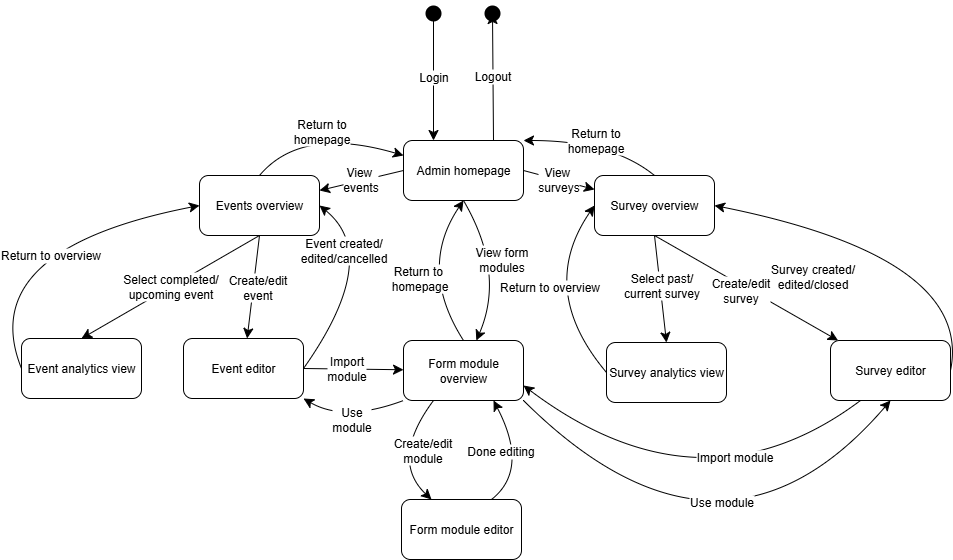
\includegraphics[width=1\linewidth]{images/state_diagram_admin.png}
    \caption{State diagram of the \gls{adm} side of the system}\label{fig:stateadmin}
\end{figure}
\end{center}

\begin{center}
\begin{figure}[H]
    \centering
    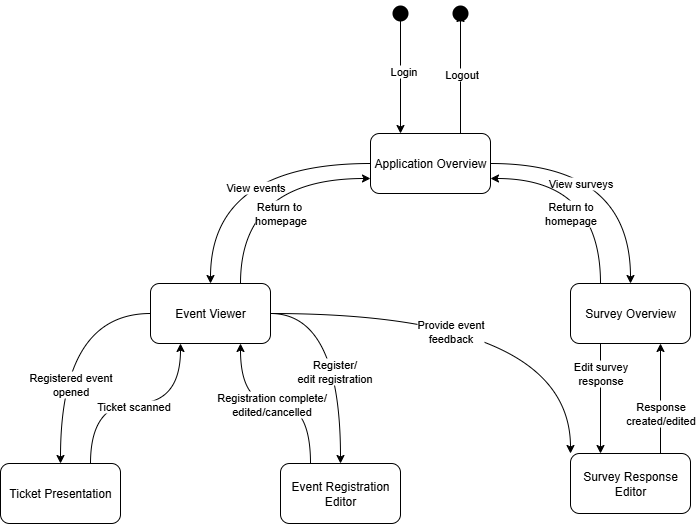
\includegraphics[width=1\linewidth]{images/state_diagram_attendee.png}
    \caption{State diagram of the \gls{atd} side of the system}\label{fig:stateattendee}
\end{figure}
\end{center}

\section{Functional Requirements}
\subsection{Functional Requirements}
\begin{enumerate}[align=left,
  leftmargin=*,
  labelsep=1em,
  itemindent=0em,
  label=\bfseries FR-\arabic*:,
  ref=\bfseries FR-\arabic*]
  \item \label{FR1} The system shall allow \glspl{adm} to create forms with multiple field types.\\[2mm]
    {\bf Motivation:} \{\textbf{G-1}, \textbf{G-5}\}. \Gls{mes} wants to be able to create forms for their surveys,
    especially \gls{cfes} surveys, with different response option types.\\
    {\bf Fit Criterion:} Forms can be created with different response styles (e.g., single choice, multiple choice,
    numeric scales) and response data is correctly stored in databases.
  \item \label{FR2} The system shall allow \glspl{adm} to organize forms for analytics, and specify how
    the analysis should be done.\\[2mm]
    {\bf Motivation:} \{\textbf{G-1}, \textbf{G-3}\}. \Gls{mes} wants to use different metrics to view survey data,
    and wants to combine multiple forms in a singular analysis.\\
    {\bf Fit Criterion:} \Glspl{adm} can combine results from multiple forms together in one analysis query, and can
    compare data points as they wish.
  \item \label{FR3} The system shall provide \glspl{atd} a method to register for events and view event information.
    \\[2mm]
    {\bf Motivation:} \{\textbf{G-2}\}. \Glspl{atd} must have a way to register for events and view event information.\\
    {\bf Fit Criterion:} \Glspl{atd} can fill out event registration forms and receive and view notifications about
    the events, and their registration is recorded in the database.
  \item \label{FR4} The system shall generate QR codes for confirmation and check-in integration.\\[2mm]
    {\bf Motivation:} \{\textbf{G-2}\}. \Glspl{atd} should be able to provide proof of registration to have easy
    access to events.\\
    {\bf Fit Criterion:} A QR code is generated and stored in the dashboard for the \gls{atd}.
  \item \label{FR5} The system shall provide an event dashboard for \glspl{adm} with filters
    for status updates on payments, waivers, event sign-ins, etc.\\[2mm]
    {\bf Motivation:} \{\textbf{G-4}\}. \Glspl{adm} must have a way to track the event and relay updates as needed.\\
    {\bf Fit Criterion:} The \gls{adm} dashboard provides trackers for sign-ins, and provides a medium to notify
    \glspl{atd} of any changes.
  \item \label{FR6} The system shall store all event data in a secure, centralized database.\\[2mm]
    {\bf Motivation:} \{\textbf{G-6}, \textbf{G-5}, \textbf{G-2}\}. Event and survey data can contain sensitive data
    from \glspl{atd}, and should only be accessed by authorized users.\\
    {\bf Fit Criterion:} Only relevant \glspl{adm} can access stored user data unrelated to their account.
  \item \label{FR7} The system shall store all questionnaire data in a secure, centralized database.\\[2mm]
    {\bf Motivation:} \{\textbf{G-1}, \textbf{G-3}, \textbf{G-6}\}. See \ref{FR6}.\\
    {\bf Fit Criterion:} See \ref{FR6}.
  \item \label{FR8} The system shall allow \glspl{adm} to generate analytics visualizations and export
    CSV/Excel reports.\\[2mm]
    {\bf Motivation:} \{\textbf{G-3}\}. \Glspl{adm} should have a way of viewing and exporting survey data.\\
    {\bf Fit Criterion:} The \gls{adm} can export queried data as CSVs or Excel-compatible files, and can view
    metrics of their choosing in the admin dashboard after specifying which metrics to plot.
  \item \label{FR9} The system shall provide event \glspl{atd} with a medium to relay feedback for the
    event.\\[2mm]
    {\bf Motivation:} \{\textbf{G-5}\}. \Gls{mes} wants to gather feedback from events and incorporate them in future
    events.\\
    {\bf Fit Criterion:} \Glspl{adm} can create feedback forms which \glspl{atd} are provided during the event which
    they can fill out, and their responses are stored in the database and are available for \glspl{adm} to access
    during or after the event.
  \item \label{FR10} The system shall provide \glspl{adm} with a medium to view all event feedback
    once an event has completed.\\[2mm]
  {\bf Motivation:} \{\textbf{G-5}, \textbf{G-4}, \textbf{G-3}\}. See \ref{FR9}.\\
  {\bf Fit Criterion:} See \ref{FR9}.
  \item \label{FR11} The system shall implement a roles-based feature access system which ensures that only relevant
    functionality and information is made available to the user.\\[2mm]
    {\bf Motivation:} \{{\bf G-4}, {\bf G-6}, {\bf G-2}\}. \Gls{mes} wants access to be restricted and ensure that
    only authorized personnel can view relevant information.\\
    {\bf Fit Criterion:} Users assigned roles can access information and features specified by those roles, and cannot
    see irrelevant features or information.
\end{enumerate}

\section{Look and Feel Requirements}
\subsection{Appearance Requirements}
\begin{enumerate}[label=LFR-AP.\arabic*, wide=0pt, leftmargin=*]
  \item The interface shall comply with \gls{mes} branding criteria (logo, colour scheme).\\[2mm]
    {\bf Motivation:} Ensures that the product is recognizable as an official \gls{mes} event registration platform.\\
    {\bf Fit Criterion:} The \gls{mes} representative shall certify that the product complies with the current standards.
  \item The tool shall have a clean, minimalist layout prioritizing the functionality.\\[2mm]
    {\bf Motivation:} Increases accessibility and user productivity, and allows for consistency across different events.\\
    {\bf Fit Criterion:} During usability testing across the \gls{mes} events, at least 80\% of students rate the forums ease of use a 4+.
  \item Admin dashboard shall clearly display relevant analytics, and distinct charts.\\[2mm]
    {\bf Motivation:} Improves organizer accessibility and readability, allowing for easier management during planning operations.\\
    {\bf Fit Criterion:} The representative shall approve of the analytics layout.
\end{enumerate}

\subsection{Style Requirements}
\begin{enumerate}[label=LFR-S.\arabic*, wide=0pt, leftmargin=*]
  \item The design shall be professional but approachable, accommodating all types of events.\\[2mm]
    {\bf Motivation:} The app should have a friendly vibe for casual student use, but maintain a sense of maturity for the more formal uses.\\
    {\bf Fit Criterion:} After use in some \gls{mes} events, 70\% of users shall agree that they trust and respect the product, and 70\% shall agree that it was not boring.
  \item The admin dashboard shall emphasize functionality and clarity, avoiding distractions just for the sake of aesthetics.\\[2mm]
    {\bf Motivation:} Admin and organizers require clear data and analytics, they have no use for stylistic components.\\
    {\bf Fit Criterion:} A sample of event organizers and club executives approve and are able to interpret all analytics without prior explanation.
\end{enumerate}

\section{Usability and Humanity Requirements}
\subsection{Ease of Use Requirements}

\begin{enumerate}[label=UHR-EoU.\arabic*, wide=0pt, leftmargin=*]
  \item Registration and feedback forms shall be easily and quickly filled out for anyone with no instruction.\\[2mm]
    {\bf Motivation:} The app should have a friendly vibe for casual student use, but maintain a sense of maturity for the more formal uses.\\
    {\bf Fit Criterion:} After use in some \gls{mes} events, 70\% of users shall agree that they trust and respect the product, and 70\% shall agree that it was not boring.
  \item Users shall sign up/sign-in to the app with no instruction. \\[2mm]
    {\bf Motivation:} The registration process is the most important aspect of the platform, so the app should have a clear and simple layout.\\
    {\bf Fit Criterion:} A sample of users shall register/login within 2 minutes without instruction.
  \item The admin dashboard shall emphasize functionality and clarity, avoiding distractions just for the sake of aesthetics.\\[2mm]
    {\bf Motivation:} Admin and organizers require clear data and analytics, they have no use for stylistic components.\\
    {\bf Fit Criterion:} A sample of event organizers and club executives approve and are able to interpret all analytics without prior explanation.
  \item The system shall provide survey progress indicators to reduce form abandonment
    rates.
\end{enumerate}

\subsection{Personalization and Internationalization Requirements}
\begin{enumerate}[label=UHR-PIR.\arabic*, wide=0pt, leftmargin=*]
  \item The custom form builder shall allow admin to create personalized forms with event-specific fields.\\[2mm]
    {\bf Motivation:} Flexibility is essential to accommodate the diverse set of events as per the scope.\\
    {\bf Fit Criterion:} The forum is used for 2 events successfully without developer assistance.
  \item Admin dashboard shall support sorting and filtering of attendees by predefined metrics.\\[2mm]
    {\bf Motivation:} Streamlines the attendee organizing process, allowing admin to categorize attendees as per the event requirements.\\
    {\bf Fit Criterion:} Organizers shall filter attendees within 1 minute of use without instruction.
\end{enumerate}

\subsection{Learning Requirements}
\begin{enumerate}[label=UHR-LR.\arabic*, wide=0pt, leftmargin=*]
  \item The app shall be easy for anyone with an intermediate level of English.\\[2mm]
    {\bf Motivation:} Users should expect intuitive, concise interactions.\\
    {\bf Fit Criterion:} 80\% of students successfully complete a form with no assistance.
  \item Admin shall be able to build a form with the custom builder with no prior instruction.\\[2mm]
    {\bf Motivation:} Event organizers are constantly changing, so it is important to reduce dependency on technical training.\\
    {\bf Fit Criterion:} 80\% of organizers shall complete a basic test form on their first attempt.
\end{enumerate}

\subsection{Understandability and Politeness Requirements}
\begin{enumerate}[label=UHR-UPR.\arabic*, wide=0pt, leftmargin=*]
  \item Basic, non-technical language will be used (Sign up instead of RSVP).\\[2mm]
    {\bf Motivation:} Increases accessibility among non-technical users, or non-fluent English speakers.\\
    {\bf Fit Criterion:} 80\% of students understand all wording without clarification.
  \item The app shall communicate errors clearly and politely.\\[2mm]
    {\bf Motivation:} Clear error messages reduce frustration and improve user experience.\\
    {\bf Fit Criterion:} Feedback suggests that 80\% of students found the experience satisfying.
  \item The app shall hide sensitive and confidential information from users.\\[2mm]
    {\bf Motivation:} Enhances security and confidence of organizations in the product.\\
    {\bf Fit Criterion:} Approval from \gls{mes} representative.
\end{enumerate}

\subsection{Accessibility Requirements}
\begin{enumerate}[label=UHR-AR.\arabic*, wide=0pt, leftmargin=*]
  \item The app shall conform to WCAG 2.1 AA standards, improving visibility for impaired users.\\[2mm]
    {\bf Motivation:} Ensures accessibility for users with visual disabilities and impairments.\\
    {\bf Fit Criterion:} Approval from a sample of students with impairments, and evaluation tools (WAVE Web Accessibility).
\end{enumerate}

\section{Performance Requirements}
\subsection{Speed and Latency Requirements}
\begin{enumerate}[align=left,
  leftmargin=*,
  labelsep=1em,
  itemindent=0em,
  label=\bfseries SL-\arabic*:]
  \item The system shall have a maximum 2-second latency for form loading, optimized for
    mobile devices.
\end{enumerate}
\subsection{Safety-Critical Requirements}
\lips
\subsection{Precision or Accuracy Requirements}
\lips
\subsection{Robustness or Fault-Tolerance Requirements}
\begin{enumerate}[align=left,
  leftmargin=*,
  labelsep=1em,
  itemindent=0em,
  label=\bfseries RF-\arabic*:]
  \item The system shall support 2047 concurrent users during peak event times.
  \item The system shall auto-save partially completed surveys every 30 seconds.
  \item The system shall recover from a server crash within 60 seconds without data loss.
  \item The system shall allow new form modules to be added without any downtime.
  \item The system shall allow \glspl{adm} to update event templates without disruption
    during ongoing events.
\end{enumerate}
\subsection{Capacity Requirements}
\lips
\subsection{Scalability or Extensibility Requirements}
\begin{enumerate}[align=left,
  leftmargin=*,
  labelsep=1em,
  itemindent=0em,
  label=\bfseries SE-\arabic*:]
  \item The system shall support up to 2047 registrations per event.
\end{enumerate}
\subsection{Longevity Requirements}
\lips

\section{Operational and Environmental Requirements}
\subsection{Expected Physical Environment}
\lips
\subsection{Wider Environment Requirements}
\lips
\subsection{Requirements for Interfacing with Adjacent Systems}
\lips
\subsection{Productization Requirements}
\lips
\subsection{Release Requirements}
\lips

\section{Maintainability and Support Requirements}
\subsection{Maintenance Requirements}
\begin{enumerate}[align=left,
  leftmargin=*,
  labelsep=1em,
  itemindent=0em,
  label=\bfseries MT-\arabic*:]
  \item The system shall provide updated documentation upon every release and be accessible to all developers\\[2mm]
    {\bf Motivation:} Allows for developers to understand the changes made on each release and will be easily be able to modify the code to fix errors or make updates. \\
    {\bf Fit Criterion:} Updated documentation will be included with the release of each version.
\end{enumerate}
\subsection{Supportability Requirements}
\begin{enumerate}[align=left,
  leftmargin=*,
  labelsep=1em,
  itemindent=0em,
  label=\bfseries SU-\arabic*:]
  \item The system shall include a FAQ section to help clarify or answer common questions.\\[2mm]
    {\bf Motivation:} Will allow for a better user experience as they can solve their own problems quickly and will make it easier for MES support teams. \\
    {\bf Fit Criterion:} Ensure a FAQ with common questions obtained from stakeholders (supervisor and MES council members) is included within the system.
\end{enumerate}
\subsection{Adaptability Requirements}
\begin{enumerate}[align=left,
  leftmargin=*,
  labelsep=1em,
  itemindent=0em,
  label=\bfseries AD-\arabic*:]
  \item The system shall run as a web app accessible through Chromium, Firefox, and Safari browsers. \\[2mm]
    {\bf Motivation:} This will allow users to use whatever browser they want and will make the application more accessible. \\
    {\bf Fit Criterion:} Test for compatibility of the application to ensure it runs on all specified browsers.
  \item The mobile app components will work on both IOS and Android platforms. \\[2mm]
    {\bf Motivation:} Allows users on both mobile ecosystems to use the app making the application more accessible. \\
    {\bf Fit Criterion:} Test the application in both the IOS and Android Environment ensuring correct functionality of all components.
\end{enumerate}

\section{Security Requirements}
\subsection{Access Requirements}
\begin{enumerate}[align=left,
  leftmargin=*,
  labelsep=1em,
  itemindent=0em,
  label=\bfseries AC-\arabic*:]
  \item The system shall require all users to authenticate using their McMaster University Email before accessing the system \\[2mm]
    {\bf Motivation:} Ensure that only the expected users of the system are using and prevent misuse from external actors.  \\
    {\bf Fit Criterion:} Allow only users who have authenticated with their emails to access the system. Ensure logs track who accesses the system and that they are authenticated.
  \item Admin level features and sensitive data are only available to users who are assigned admin roles. \\ [2mm]
    {\bf Motivation:} Prevents unauthorized users from viewing sensitive event and user data.  \\
    {\bf Fit Criterion:} Perform testing to ensure that features deemed to be admin-level are only accessible to the users who are given those roles. Ensure that data is only accessible to admins
\end{enumerate}
\subsection{Integrity Requirements}
\begin{enumerate}[align=left,
  leftmargin=*,
  labelsep=1em,
  itemindent=0em,
  label=\bfseries IG-\arabic*:]
  \item The system shall provide input validation for all user submitted data \\[2mm]
    {\bf Motivation:} Ensures the safety of our application by ensuring only the required input types are entering our database. Protects us from SQL injection and data corruption in our database.  \\
    {\bf Fit Criterion:} All inputs will include checks to ensure only the correct type is entering our database. Perform testing to ensure that all inputs have validation checks.
  \item The system shall only use HTTPS for communication between clients and servers \\[2mm]
    {\bf Motivation:} Ensures a secure connection between our client and server and protects against the interception or tampering of data during data transmission. \\
    {\bf Fit Criterion:} All requests will be done through HTTPS and if an HTTP request is done we will redirect it to HTTPS. \\
\end{enumerate}
\subsection{Privacy Requirements}
\begin{enumerate}[align=left,
  leftmargin=*,
  labelsep=1em,
  itemindent=0em,
  label=\bfseries PV-\arabic*:]
  \item Users shall have the ability to request for the deletion of their stored personal data\\[2mm]
    {\bf Motivation:} Increases transparency and control over their own data for users. Provides reassurances for users that their data can be removed if neccesary.    \\
    {\bf Fit Criterion:} Ensure a mechanism exists for users to delete their data. Peform testing so that the mechanism actually removes all related data from the database.
  \item The system shall only store sensitive data after obtaining the consent of the user \\[2mm]
    {\bf Motivation:} Keeps us legally sound as we are not storing user data without first obtaining consent. Also provides users with information on what their data is actually being used for.  \\
    {\bf Fit Criterion:} Ensure that all sections which require inputting sensitive information have consent checks where we explicitly explain what is being stored and how it may be used. \\
  \item All sensitive user information such as student numbers, names and emails shall be encrypted in storage using AES-256\\[2mm]
    {\bf Motivation:} Protects user's information from unauthorized viewing and ensures that even if a breach were to occur sensitive information will not be leaked.   \\
    {\bf Fit Criterion:} Inspect database to show that the required fields are stored encrypted and not in plaintext. \\
\end{enumerate}
\subsection{Audit Requirements}
\begin{enumerate}[align=left,
  leftmargin=*,
  labelsep=1em,
  itemindent=0em,
  label=\bfseries AU-\arabic*:]
  \item The system shall track admin action inside an audit log\\[2mm]
    {\bf Motivation:} Ensures traceability of admin actions and allows other admins to know who performed what.  \\
    {\bf Fit Criterion:} 100\% of actions will be in a log with tracking of user who did the action, timestamp and action commited. Testing will be done to ensure all actions are being logged and logs should be exportable for review.
\end{enumerate}
% \subsection{Immunity Requirements}
% \textit{No relevant requirements}

\section{Cultural Requirements}
\subsection{Cultural Requirements}
\begin{enumerate}[align=left,
  leftmargin=*,
  labelsep=1em,
  itemindent=0em,
  label=\bfseries CL-\arabic*:]
  \item The system shall use Canadian English spelling.\\[2mm]
    {\bf Motivation:} \Gls{mes} is an organization located in Canada.\\
    {\bf Fit Criterion:} All rendered text provided by the system passes a Canadian English spell-checker.\\
\end{enumerate}

\section{Compliance Requirements}
\subsection{Legal Requirements}
\begin{enumerate}[align=left,
  leftmargin=*,
  labelsep=1em,
  itemindent=0em,
  label=\bfseries LG-\arabic*:]
  \item The system shall store and handle all sensitive personal data in compliance with PIPEDA regulations.\\[2mm]
    {\bf Motivation:} The system will store private personal information, which must be done responsibly.\\
    {\bf Fit Criterion:} The system meets all PIPEDA regulation requirements.\\
\end{enumerate}
\subsection{Standards Compliance Requirements}
\begin{enumerate}[align=left,
  leftmargin=*,
  labelsep=1em,
  itemindent=0em,
  label=\bfseries ST-\arabic*:]
  \item The system code shall conform to the \textit{Airbnb JavaScript Style Guide} and \textit{Airbnb React/JSX
    Style Guide}.\\[2mm]
    {\bf Motivation:} Specified in Development Plan \S \ 11.\\
    {\bf Fit Criterion:} The system code passes all CI/CD checks related to formatting compliance.\\
\end{enumerate}

\section{Open Issues}
There are currently no open issues which need to be considered at this stage of the development cycle.
% Any problems that remain unresolved and undefined
\section{Off-the-Shelf Solutions}
\subsection{Ready-Made Products}
There are some products that exist on the market which solve certain components of this product but no product exists
that combines these components into one. For event management there are various tools such as EventBrite and Stubhub
which can allow for the selling of tickets for events. The problem with these products are that they don't integrate
well with current \gls{mes} Systems and don't provide all the features as required such as collecting waivers and
ensuring McMaster students attend university specific events. For general data collection Google Forms is the most used
tool, and it allows for the creation of complex forms and stores data in spreadsheets. For further data analysis it
requires effort on the part of the form creator to actually go and analyze the data to gain actual insights. Also, the
forms can become hard to handle as they become complex and can become confusing for respondents. As mentioned before
there is no tool that has a combination of the two components.
\subsection{Reusable Components}
There are various components that we can use to help develop our application:
\begin{itemize}
  \item \textbf{Vite}: Provides us with a framework for developing web apps in \textbf{React} and provides built in
    routing behaviour. It also handles many built in libraries and packages that we can use for front-end styling such
    as \textbf{tailwind-css}. We can also integrate it with other libraries for authentication and for database
    management
  \item \textbf{TanStack}: Provides us with a powerful middleware to connect backend and front-end services. Will
    primarily be used for routing but also offers data visualization capabilities. Offers many libraries for working
    with data and state management that we can leverage.
  \item \textbf{SurveyJS}: This is a potential tool we can use to develop the form builder as it provides us with some
    pre-built components we can use to develop and customize our own forms.
  \item \textbf{Recharts}: This could be potential charting tool we can use to develop our admin dashboard. Though there
    are other charting tools the benefit of Recharts is that it provides customization on top of the pre-built charts.
  \item \textbf{Drizzle}: We can use Drizzle as an ORM to map from our database to our web-app. Drizzle is useful since
    it is lightweight and is code first. Drizzle's simplicity allows for faster development and is perfect for our use
    case.
\end{itemize}
These components will allow us to develop our application faster and more efficiently as many of these products are
already optimized. All the above products are free to use so do not incur any extra costs or require the handling of
licenses.
\subsection{Products That Can Be Copied}
\textit{There don't seem to be any products that can be copied which contain all the required components within a single
product. Moreover, the \gls{mes} wants a product that doesn't require an external license and wants to be fully built in
house, so they have control over future development and usage.}

\section{New Problems}
\subsection{Effects on the Current Environment}
\lips
\subsection{Effects on the Installed Systems}
\lips
\subsection{Potential User Problems}
\lips
\subsection{Limitations in the Anticipated Implementation Environment That May
Inhibit the New Product}
\lips
\subsection{Follow-Up Problems}
\lips

\section{Tasks}
\subsection{Project Planning }

\begin{itemize}
    \item \textbf{Task Assignment:} Tasks are divided based on each member’s technical strengths and defined roles.
    Rayyan leads the admin web UI, Virochaan handles full-stack web and DevOps, Ibrahim focuses on backend and mobile integration, Omar develops mobile UI components, and Mahdi manages backend logic and database design.
    \item \textbf{Collaboration:} Weekly meetings are held to review progress, plan upcoming work, and prepare for supervisor syncs.
    Daily communication occurs over Discord, while GitHub Issues serve as the main hub for technical updates.
    \item \textbf{Quality Control:} All new code must pass automated linting and testing via GitHub Actions before merging.
    Peer reviews on pull requests ensure consistency and prevent regressions.
\end{itemize}

\subsection{Planning of Development Phases}

Development is organized into five phases, each with clear goals and deliverables.
The primary objective is to have a fully functional \textbf{Minimum Viable Product (MVP)} by the end of \textbf{December 2025}, where all four core features work at a basic level before refinement begins.

\begin{enumerate}
    \item \textbf{Phase 1 – Requirements and Design (September–October 2025)}
    Finalize system requirements, architecture, and UI mockups for the Admin Portal and Custom Form Builder.
    Deliverables include the SRS, Hazard Analysis, and shared API specifications with Projects B and C.

    \item \textbf{Phase 2 – Core Functionality and MVP (Mid October–December 2025)}
    Implement the main system features for a working MVP:
    \begin{itemize}
        \item Basic \textbf{Custom Form Builder} for creating and saving modular forms.
        \item Functional \textbf{Registration and Feedback Forms} linked to the backend.
        \item Simple \textbf{Attendee Overview Dashboard} showing registration data.
        \item Initial \textbf{Backend Analytics} for event and submission counts.
    \end{itemize}
    The MVP will demonstrate a complete flow—from form creation to submission and viewing results.

    \item \textbf{Phase 3 – Integration and Refinement (January 2026)}
    Improve performance, UI/UX, and backend data handling.
    Begin integration testing with Projects B and C to ensure smooth database and API interaction.

    \item \textbf{Phase 4 – Analytics and Dashboard Expansion (February–March 2026)}
    Enhance analytics and administrative tools with filtering, charts, and export options (CSV/PDF).
    The dashboard will evolve into a production-ready tool for MES event organizers.

    \item \textbf{Phase 5 – Testing and Deployment (March–April 2026)}
    Conduct final testing, bug fixes, and documentation updates.
    Complete cross-team integration and deploy the system for real MES events such as Fireball Formal or CALE Conference.
    Prepare final deliverables and the Capstone Expo presentation.
\end{enumerate}

\section{Migration to the New Product}
\subsection{Requirements for Migration to the New Product}
\lips
\subsection{Data That Has to be Modified or Translated for the New System}
\lips

\section{Costs}
We don't expect any costs to arise during the development of the project. We will be using free tools and libraries for
development and for hosting we will look to host databases and the back-end locally. In production the hosting will be
done by the \gls{mes}, so it is out of the scope of this Capstone.

\section{User Documentation and Training}

\subsection{User Documentation Requirements}

No separate written documentation or manuals are planned for this system.
Instead, all user guidance will be built directly into the application to create a more natural and seamless learning experience.
This approach ensures that both attendees and administrators can quickly understand how to use the platform without leaving the interface.

The system will include:
\begin{itemize}
    \item \textbf{Interactive Onboarding:}
    Step-by-step tutorial pop-ups and tooltips that appear during first-time use to introduce users to key features such as event registration, check-in, and analytics.

    \item \textbf{Guided Walkthroughs:}
    Contextual highlights that show users where to click and how to complete common actions directly within the interface.

    \item \textbf{Short Visual Aids:}
    Optional embedded videos or animations explaining how to perform important tasks, such as creating an event or submitting a form.
\end{itemize}

These interactive elements replace the need for formal documentation and are designed to make the system self-explanatory and easy to learn.
Users will be able to replay the onboarding sequence or revisit tips at any time from within the application.

\subsection{Training Requirements}

No formal training sessions or written instructions are required for this system.
The design prioritizes simplicity, discoverability, and self-learning through interactive guidance.

\begin{itemize}
    \item \textbf{End Users (Attendees):}
    Will learn the system through in-app pop-ups and short guided tutorials shown during their first login.
    These tutorials will walk users through tasks such as signing up for an event, filling out a form, or checking in.

    \item \textbf{Administrators and Event Organizers:}
    Will be guided through core management workflows using the same interactive approach, supported by optional short videos or animations that explain advanced features such as creating forms or viewing analytics.
\end{itemize}

Overall, training and documentation will be fully integrated into the user experience.
The application itself will serve as the guide, helping users learn by doing rather than reading external instructions.


\section{Waiting Room}

This section outlines extra features to consider that may or be not be implemented depending on time constraints.

\begin{enumerate}[align=left,
  leftmargin=*,
  labelsep=1em,
  itemindent=0em,
  label=\bfseries WR-\arabic*:,
  ref=\bfseries WR-\arabic*]
  \item \label{WR1} The entire system shall be redistributable, customizable, and deployable for use by any organization. \\[2mm]
    {\bf Motivation:} The system being built for the \gls{mes} can be expanded into a Software-as-a-Service (SaaS) for any organization looking for a centralized event or survey management system. \\
    {\bf Fit Criterion:} At least two isolated copies of the system should be able to run simultaneously without any connections or interference between systems.
  
  \item \label{WR2} All forms of branding in the system shall be substitutable for a different branding through an easily accessible interface.\\[2mm]
  {\bf Motivation:} If the system shall be expanded for use by any organization, the organization should be able to customize all branding of the system without requiring changes to the source code.\\
  {\bf Fit Criterion:} All \gls{mes} branding should be removable and replaceable with seperate branding throughout the \gls{adm} and \gls{atd} systems without making any edits to source code.

  \item \label{WR3} The system shall allow for live polling of all \glspl{atd} registered for a given event. \\[2mm]
  {\bf Motivation:} Allowing for live polling of \glspl{atd} during an event can increase \gls{atd} engagement and further integrate the \gls{mes}'s suite of required tools into the centralized system\\
  {\bf Fit Criterion:} The feature shall be tested during an event with at least 10 registered \glspl{atd}. All registered \glspl{atd} should receive the poll, submit a reponse, and an \gls{adm} shall be able to view all reponses within 5 minutes.

  \item \label{WR4} The system shall provide the \gls{adm} with a report of recommendations to improve survey reponse rates and event turnout.\\[2mm]
  {\bf Motivation:} Improving event turnout and survey reposnse rates is one of the main goals of the \gls{mes} for the proposed system. Adding intelligent recommendations based on previous survey and event data to improve this will increase the satisfaction of associated stakeholders.\\
  {\bf Fit Criterion:} Upon creation of an event or survey, the system should inform the \gls{adm} of at least one parameter that can be changed to improve event turnout or response rates.

  \item \label{WR5} The system shall provide the \gls{adm} with a reasonable prediction of the turnout of any given event.\\[2mm]
  {\bf Motivation:} Predicting the turnout of an event can better prepare the \gls{mes} for event planning, finance management, and resource allocation.\\
  {\bf Fit Criterion:} Upon creation of an event, the system should inform the \gls{adm} of the predicted turnout of the event that is within 20\% of the actual turnout.
  
\end{enumerate}


\section{Ideas for Solution}
\lips

\newpage{}
\section*{Appendix --- Reflection}

The purpose of reflection questions is to give you a chance to assess your own
learning and that of your group as a whole, and to find ways to improve in the
future. Reflection is an important part of the learning process.  Reflection is
also an essential component of a successful software development process.  

Reflections are most interesting and useful when they're honest, even if the
stories they tell are imperfect. You will be marked based on your depth of
thought and analysis, and not based on the content of the reflections
themselves. Thus, for full marks we encourage you to answer openly and honestly
and to avoid simply writing ``what you think the evaluator wants to hear.''

Please answer the following questions.  Some questions can be answered on the
team level, but where appropriate, each team member should write their own
response:



\subsubsection*{Group Reflection}
\begin{enumerate}
  \item \textbf{How many of your requirements were inspired by speaking to your client(s) or their proxies (e.g. your peers, stakeholders, potential users)?}
  Most of our functional requirements were obtained directly through conversations with out supervisor (Luke) or through todcumentation provided by him. This provided us with a good starting point on what his vision of the system would look like and from there we built upon and added requiremnts based on what we throught the system needed.

  \item \textbf{Which of the courses you have taken, or are currently taking, will help your team to be successful with your capstone project.}
  \begin{itemize}
      \item SFWRENG 4HC3: This course will help us design the frontend components and create a platform which will provide a positive user experience.
      \item SFWRENG 3DB3: Help us design effective database schema and queries.
      \item SFWRENG 3A04: This will help us design our architecture for the system. Also gave us experience working with git control and designing sytem with diagrams.
      \item SFWRENG 2AA4: Designing full scale software and using github project management.
      \item ENG 3PX3 + 2PX3: This course gave us some basic project and team management skills as we had to work on semester long projects similar to what is being done in this course.
      \item SFWRENG 3RA3: Gave us help writing this document and will help us refine and update our requirements in the future.
      \item SFWRENG 3S03: Develop test cases to ensure that our code is working as intended and to allow for CI since we can ensure subsequent changes don't break the whole system.
  \end{itemize}

  \item \textbf{What knowledge and skills will the team collectively need to acquire to successfully complete this capstone project?  Examples of possible knowledge to acquire include domain specific knowledge from the domain of your application, or software engineering knowledge, mechatronics knowledge or computer science knowledge.  Skills may be related to technology, or writing, or presentation, or team management, etc. You should look to identify at least one item for each team member.} \\
  \begin{enumerate}
    \item Full-Stack Web Development: Some skills in this category that will be needed to be learned include requiring the development of front-end and UI. We also need to to develop apis with the restful architecture to connect back-end with our front-end framework. As seen in our document our tech stack includes Vite, React and TanStack Router. These are new technologies to use which we will have to learn.
    \item Software QA and Testing: Using CI/CD to ensure that our code meets the standards that we set and doesn't break when pushing to production. Develop Test Cases to ensure that all code is working as intended and with CI ensure that it automatically is run on each iteration we push to the repository.
    \item Frontend + UI Design: We need to design good user interfaces to ensure that our application will be intuitive to use and will provide users with a positive experience,
    \item Database Management and Design + Data analytics: Create database schema and sql queries to generate and visualize basic data analytics and dashboards.
    \item Software Architecture and Design: Develop an architecture that allows for expandability past the term of our project. We need to acquire skills on different software designs which will allow for better scalability in the future.
    
  \end{enumerate}
  \item \textbf{For each of the knowledge areas and skills identified in the previous question, what are at least two approaches to acquiring the knowledge or mastering the skill?  Of the identified approaches, which will each team member pursue, and why did they make this choice?} \\
  \begin{enumerate}
    \item To acquire this skill we can look to look at the documentation for the technologies. Vite and TanStack have well written documentation on how the framework works as well as how to integrate these frameworks with other technologies we will use in the project. There are also many tutorials and example full-stack projects found on github and accross the internet. Looking at these projects we could gain to understand how to properly implement these technologies and best practices for coding with these frameworks. \\
    \\
    \textbf{Virochaan} and \textbf{Omar} will be looking to improve their skills and knowledge of this domain. Virochaan has past experience working in full-stack development in his co-op so he will be looking to build upon that by using the approaches mentioned above. Omar has been interested in Full-Stack development and has worked on personal projects in this field. He will be looking to transfer the skills he has learnt and use them with these new technologies.\\
    \item To acquire this knowledge we can look back on past courses we did and utilize the testing techniques and methods used in those courses. We can also practice by conducting group peer review sessions of our code and implementing test cases on previous projects and assignments we may have done. \\
    \\
    \textbf{Rayyan} and \textbf{Mohammad} will be looking to improve their skills and knowledge in this domain. Both Rayyan and Mohammad have skills in ths area through past co-op experiences and excelled in the testing course in 3rd year. Mohammad is looking to improve his skills in this category as he believes that this is a useful skill to have for he future career and something he wants to master.
    \item To acquire these skills we can review front-end design principles from our Human-Computer Interaction course and research UI/UX design guidelines. We can also use design tools such as \textit{Figma} to create low-fidelity and high-fidelity mockups of our interfaces before implementing them in code. \\
    \\
    \textbf{Virochaan} and \textbf{Ibrahim} will be looking to improve their skills and knowledge in this domain. Virochaan is interested in improving his skills in this area because he feels that he is weak in this field and finds that having these skills will make him more well-rounded developer. Ibrahim is interested in both full-stack and front-end design and finds that this could be a good experience to gain more exposure in this area.  
    \item  We can use the PostgreSQL documentation and online tutorials to deepen our understanding of how to properly utilize this technology. We can also watch videos on general relational database management as well as effective indexing and querying to make our databases as efficient as possible. 
    \\
    \textbf{Rayyan} and \textbf{Ibrahim} will be looking to improve their skills and knowledge in this domain. Rayyan has experience working on this field in his co-op and found it to be a fulfilling experience. He wants to build upon that foundation and gain more skills working on databases to make him a better back-end developer. Ibrahim perfomed well in the databases course in 3rd year and believes that this could be a good way to build upon that. He always wanted to work on the back-end and database for this project and believes that gaining skills in this area will make him more prepared to accomplish this.\\
    \item To acquire this skill we can study various architectural patterns such as Model-View-Controller (MVC) and Layered Architecture, which are suitable for scalable web systems. We will review course materials from SFWRENG 3A04 and examine open-source project repositories to understand how modular designs are structured. We can also use diagramming tools to model the architecture of our own system before implementation to familiarize ourselves with them. \\
    \\
    \textbf{Omar} and \textbf{Mohammad} will be looking to improve their skills and knowledge in this domain. Omar wishes to pursue this since he wishes to build upon skills he learned in 3A04. In his co-op he had experience working with the MVC architecture and is looking to develop his skills in this area to learn about more patterns. Mohammad also had experience working various architecture types at his co-op. He is looking to put to practice what he learned there in this project while building upon his skillset.
  \end{enumerate}
\end{enumerate}

\subsubsection*{Virochaan Ravichandran Gowri Reflection}
\begin{enumerate}
  \item \textbf{What went well while writing this deliverable?} \\
  During the writing of this deliverable we all had a clear understanding of the goals of this project and the general
  plan which we did in the past deliverable. From this through conversations with our supervisors we were easily able to
  obtain requirements that were relevant to our project. The best part was the communication between the members of our
  team and with the supervisor. This allowed us to
  \item \textbf{What pain points did you experience during this deliverable, and how did you resolve them?} \\
  We needed to make sure that we remained flexible in our requirements if we had to make changes in the future. This was
  especially crucial because we knew that there could be a chance that there could be additional requirements or changes
  based on what the client wanted. Also the client wanted a certain stack so we didn't really have flexibility regarding
  that so it was some new technologies that we need to become accustomed with.

\end{enumerate}

\subsubsection*{Mohammad Mahdi Mahboob Reflection}
\begin{enumerate}
  \item \textbf{What went well while writing this deliverable?} \\
  The projects constraints section write-up went smoothly. Due to previous meetings with the client as well as
  documentation outlined in previous deliverables, much of the constraints were readily available and thereby easily
  articulable. Most constraints regarding the environment of the solution as well as specific requests were
  well-documented in our communications with the client; their technical aptitude was greatly appreciated since they
  were able to provide us with a clear technology and development roadmap to facilitate collaboration across Capstone
  groups for the integrated application.
  \item \textbf{What pain points did you experience during this deliverable, and how did you resolve them?} \\
  Some pain points I encountered during this deliverable were encountered when articulating the requirements. It was
  difficult to gauge what an appropriate level of granularity would be for some of the requirements, as well as decide
  whether requirements for some subsections were necessary. Defining fit criteria was also difficult at times,
  especially for requirements which related to the internal behaviour of the system, such as FR-11. In order to resolve
  these discrepancies, I consulted my teammates and brought forth these concerns during supervisor meetings to
  clarify details, as well as explicitly ascertain the relevance of different requirement categories, such as
  compliance. I would like to commend my teammates in this regard, as well as thank our supervisor for their time and
  expertise.
\end{enumerate}
\subsubsection*{Rayyan Suhail Reflection:}
\begin{enumerate}
  \item \textbf{What went well while writing this deliverable?} \\
  I worked on the Purpose, Relevant Facts and Assumptions, New Problems, Tasks, Migration, and User Documentation sections. What went well was how everything started connecting once we finalized our project direction. Writing the User Documentation section was interesting since we focused on in-app guidance instead of long manuals. The planning sections also came together nicely after a few team discussions, and overall, our communication made the process much smoother.

  \item \textbf{What pain points did you experience during this deliverable, and how did you resolve them?} \\
  The main challenge was keeping the document consistent and not too repetitive across similar sections. Some template areas, like Migration and New Problems, were tricky to adapt to our system at first. I resolved this by reviewing past SRS examples and working closely with my teammates to make sure our sections aligned and stayed concise.
\end{enumerate}







\end{document}
